\documentclass[10pt]{article}
\usepackage[polish]{babel}
\usepackage[utf8]{inputenc}
\usepackage[T1]{fontenc}
\usepackage{graphicx}
\usepackage[export]{adjustbox}
\graphicspath{ {./images/} }
\usepackage{amsmath}
\usepackage{amsfonts}
\usepackage{amssymb}
\usepackage[version=4]{mhchem}
\usepackage{stmaryrd}

\begin{document}
\begin{center}

\includegraphics[max width=\textwidth]{2024_11_21_6d30b4190bf1b57758c7g-1}
\end{center}

\begin{enumerate}
  \item Liczbę 2019 przedstaw w postaci różnicy dwóch kwadratów liczb naturalnych. Podaj wszystkie rozwiązania i uzasadnij, że nie ma więcej.
  \item Wykaż, że jeśli \(a\) i \(b\) są takimi liczbami dodatnimi, że \(a \cdot b \geq a+b\), to \(a+b \geq 4\).
  \item W trójkącie \(A B C\) odcinek \(A F\) jest środkową, \(D-\) środkiem odcinka \(A F, E\) punktem przecięcia prostej \(C D\) i boku \(A B\). Ponadto wiadomo, że \(B D=B F=C F\). Udowodnij, że \(A E=D E\).\\
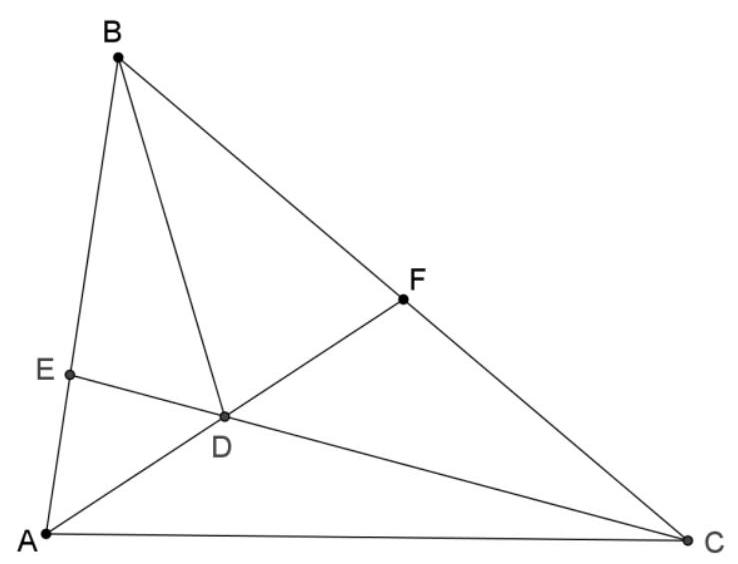
\includegraphics[max width=\textwidth, center]{2024_11_21_6d30b4190bf1b57758c7g-1(1)}
\end{enumerate}

\end{document}